The followed informations introduce the results of two different tests 
using the KITTI dataset\cite{Geiger}.


In the first test in Fig. \ref{fig:imgpapercerta}, 
the algorithm makes the tracking of an object through nine images in sequence with 
a displacement approximately perpendicular to the observer.
\begin{figure}[!hbt]
\centering
  \subfloat[]{\label{fig:imgpapercertaa} 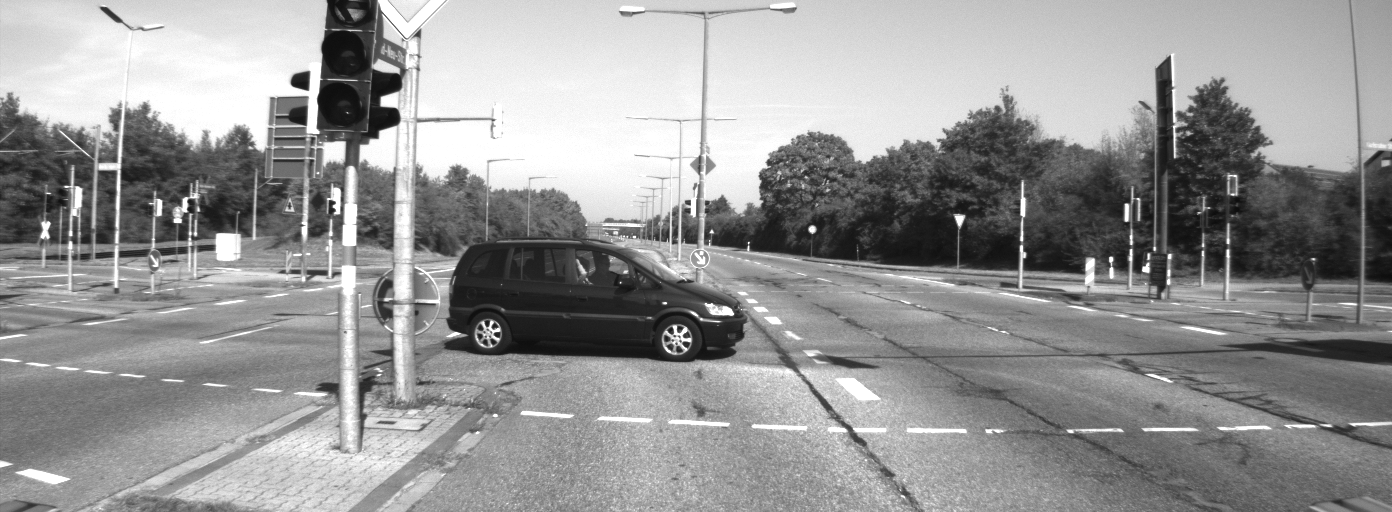
\includegraphics[width=.48\columnwidth]{images/images/0000000000.png}}
  \subfloat[]{\label{fig:imgpapercertab} 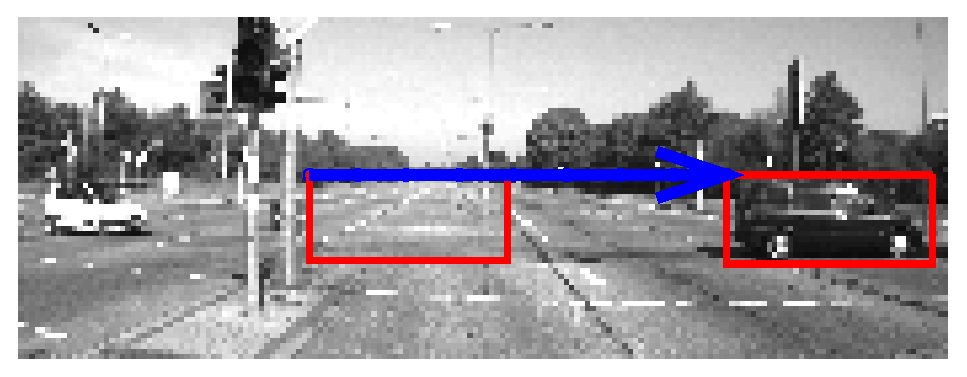
\includegraphics[width=.48\columnwidth]{images/images/img_paper_certa.eps}}
  \caption{The image in (a) represents the target in its initial position 
   and the image (b) shows the vehicle in its final position.}
  \label{fig:imgpapercerta}
\end{figure}
The initial position of target is in the image (a) and the final position in (b), 
where a vector (in blue) illustrates the resulting trace.
We can observe that there is a small bend in the image 
and it generates a slight change of object perspective. 
This cause the update of the $ROI$, which involves seeing a slight change in area.
The difference among the initial and final values of the departure factor may 
be considered small, as shown in Fig. \ref{fig:res_graph1}.
\begin{figure}[!hbt]
\centering
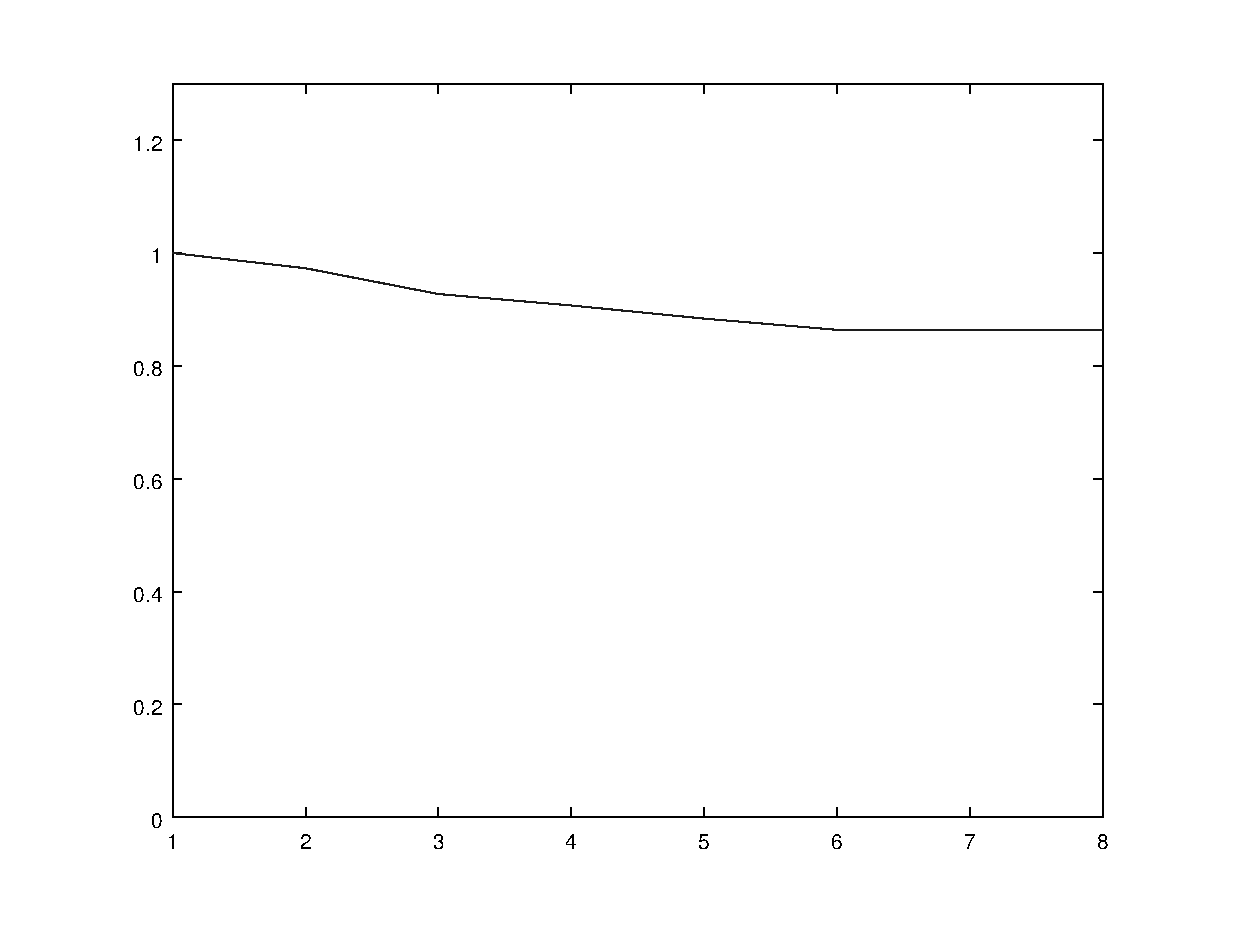
\includegraphics[width=0.8\columnwidth]{images/graph1.eps}
\caption{Departure factor for each frame in the test 1.}
\label{fig:res_graph1}
\end{figure}
Fig. \ref{fig:res_graph1v} shows the velocity of departure factor
to a value $d_0=1$ and a $\Delta t=1$. It demonstrates that the variation
of the departure factor is very small when compared with 1. 
It has a mean departure factor (velocity) of $-0.017020$. This implies in a mean approach of $1.7\%$ of $d_0$
in each one of the nine frames.
\begin{figure}[!hbt]
\centering
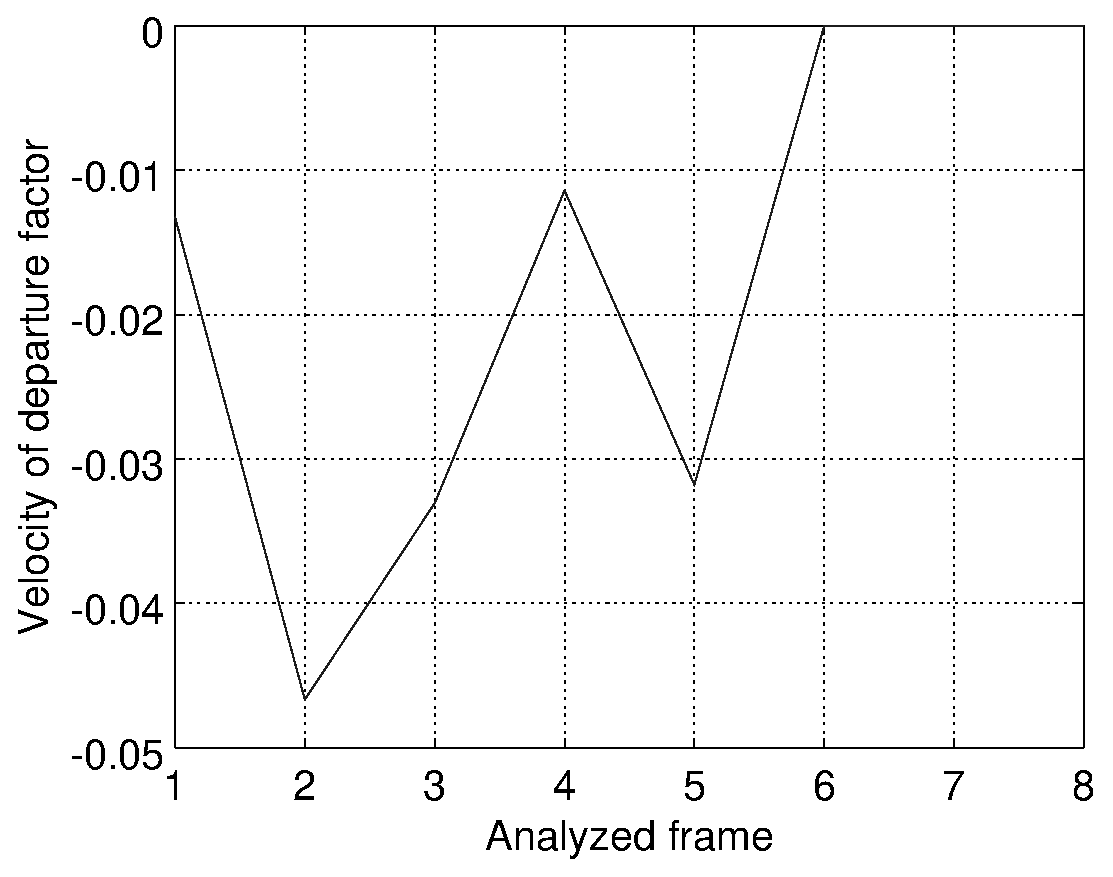
\includegraphics[width=0.8\columnwidth]{images/graph1v.eps}
\caption{Velocity of departure factor for each frame in the test 1.}
\label{fig:res_graph1v}
\end{figure}


In the second test, we prove the functionality of the algorithm in three dimensions. 
The algorithm compares the images and calculates the departure factor 
based on the target area. Fig. \ref{fig:target} demonstrates the 
tracking of $100$ images from initial position to the final position of the target, 
highlighted with red boxes;
where, the vector in blue describes the movement of the target. 
\begin{figure}[!hbt]
\centering
  \subfloat[]{\label{fig:targeinit} 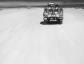
\includegraphics[width=.48\columnwidth]{images/images/351.jpg}}
  \subfloat[]{\label{fig:targeend} 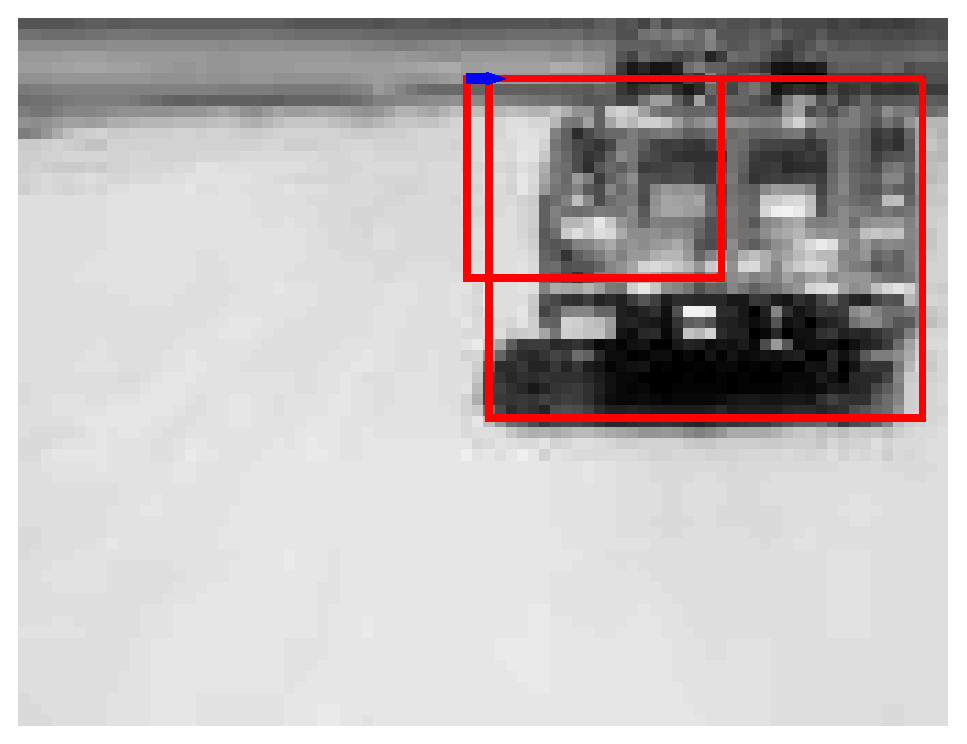
\includegraphics[width=.48\columnwidth]{images/graph2p.eps}}
  \caption{The target in (a) is the initial position and its area is smaller than the target in (b), 
  which represents the final position. The factor is dividing both areas.}
  \label{fig:target}
\end{figure}
In Fig. 8, we can observe a significant increase in the target area, and 
its influence to the departure factor is shown in Fig. \ref{fig:res_graph2}.

\begin{figure}[!hbt]
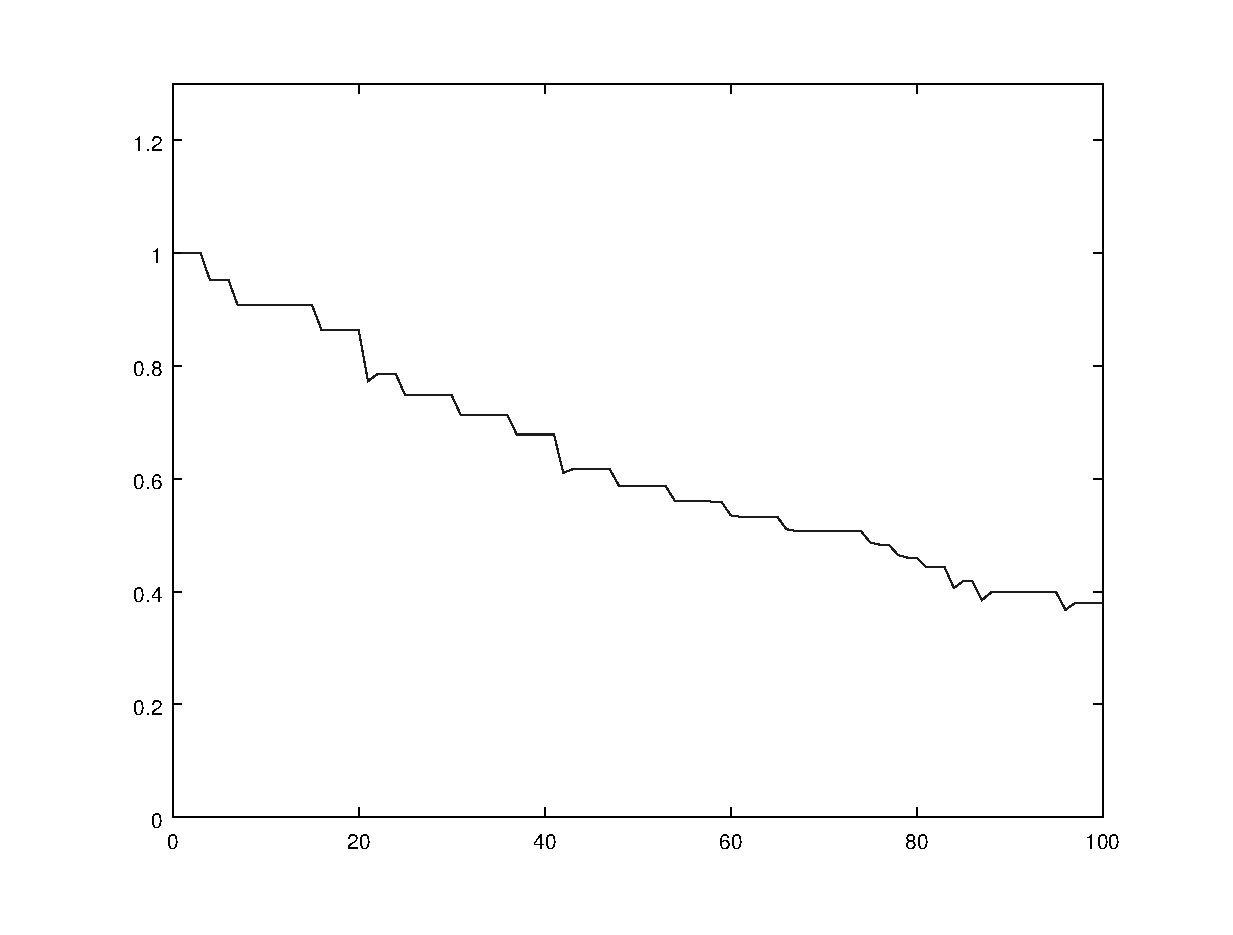
\includegraphics[width=\columnwidth]{images/graph2.eps}
\caption{Departure factor for each frame in the test 2.}
\label{fig:res_graph2}
\end{figure}
The Fig 9 shows the departure factor in each frame
in test 2. If we interpret this value as the position in each sample time, 
then the departure factor describes the relative target position.
In the first image the analyzed target is at a distance $d_0$ 
and in the last image the target is at a distance of $52.42\%$ of $d_0$.
The departure distance decreases in discrete steps because the departure
factor is selected in discrete steps, if the target is
between two consecutive analysis layers (scales), the algorithm
approximates the target to the nearest layer. 
\begin{figure}[!hbt]
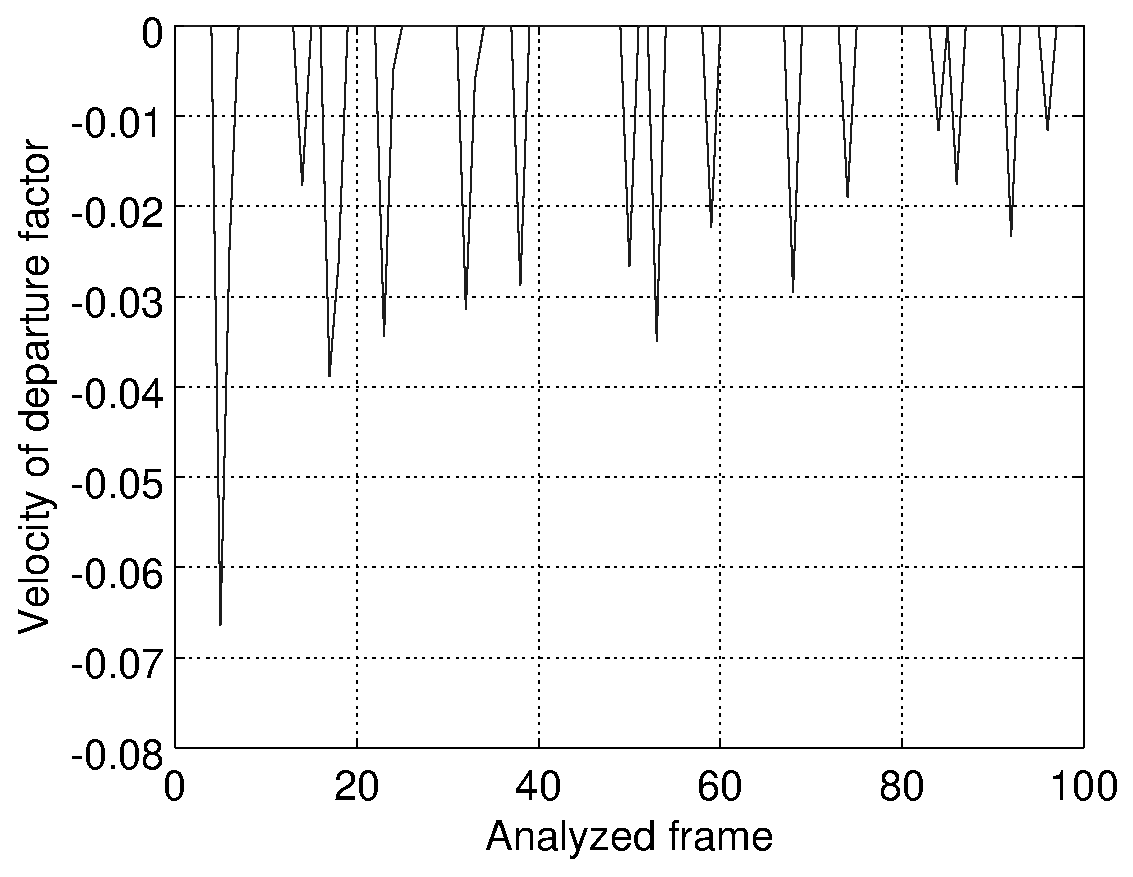
\includegraphics[width=\columnwidth]{images/graph2v.eps}
\caption{Velocity of departure factor for each frame in test 2.}
\label{fig:res_graph2v}
\end{figure}
On the other side, the velocity of departure factor is shown in 
Fig. \ref{fig:res_graph2v}, where the velocity is calculated
to $d_0=1$ and $\Delta t=1$. The mean value of the departure
velocities is equal to $-0.0048$, which indicates that the
analyzed object is in approaching towards the observer. Similar
to the case of test 1, this mean velocity can be interpret
as a mean approach of $0.48\%$ of $d_0$, in each one of 100 frames.
If we compare test 1 and 2 to the same $\Delta t=1$, it is evident 
that the departure velocity of  test 2  is lower than  test 1, 
but as  test 2 has more analysed frames (100 images)
and because this the approaching to the observer is greater; 
not to mention that in test 1, the small number of images 
make  unrepresentative the mean value.




